\section{Besoins Métier}

%
%
\subsection{Contexte}

On se situe dans le cadre d'un établissement hospitalier, une clinique, qui souhaite développer une offre médicale dédiée aux maladies des voies respiratoires.
Pour cela un nouveau pôle est construit à 50 mètres du bâtiment déjà existant de la clinique.
Nous sommes chargés de réaliser l'étude de l'architecture réseau à implanter dans ce nouveau bâtiment.

%

Ce réseau devra répondre à une certaine tolérance aux pannes puisque utilisé à des fins médicales.
Une interconnexion avec le bâtiment adjacent sera aussi nécessaire.
Dans l'architecture réseau actuelle le cœur de réseau et l'accès à Internet se trouvent dans le bâtiment adjacent.
Le déploiement de la nouvelle portion de réseau ne devra avoir aucune incidence sur le réseau déjà existant de la clinique.
Les dimensions du bâtiment sont d'environ 35 mètres de long pour 11 mètres de large.
Il est composé de 6 étages ayant chacun différents usages.
Les différences entre ces étages seront un point de départ important pour établir l'architecture réseau : par exemple certains équipements médicaux nécessitent d'être inter-connectés, d'autres ne doivent en aucun cas être parasités pour assurer leur fonctionnement.

%

L'objectif principal est d'assurer un service performant, péren et sécurisé tant pour le personnel que pour les patients.
Le réseau d'un hôpital ne dispose pas spécialement de performances de débit minimum mais demande une stabilité, une haute disponibilité et une sécurité très importante.
Plusieurs solutions peuvent répondre à ce cahier des charges en respectant les critères suivants, nous proposerons la solution qui nous parait la plus adaptée à cette situation :
\begin{itemize}
\item La fiabilite ;
\item Le coût ;
\item La sécurité ;
\item La durée de mis en place.
\end{itemize}

%

\begin{figure}[!ht]
    \center
    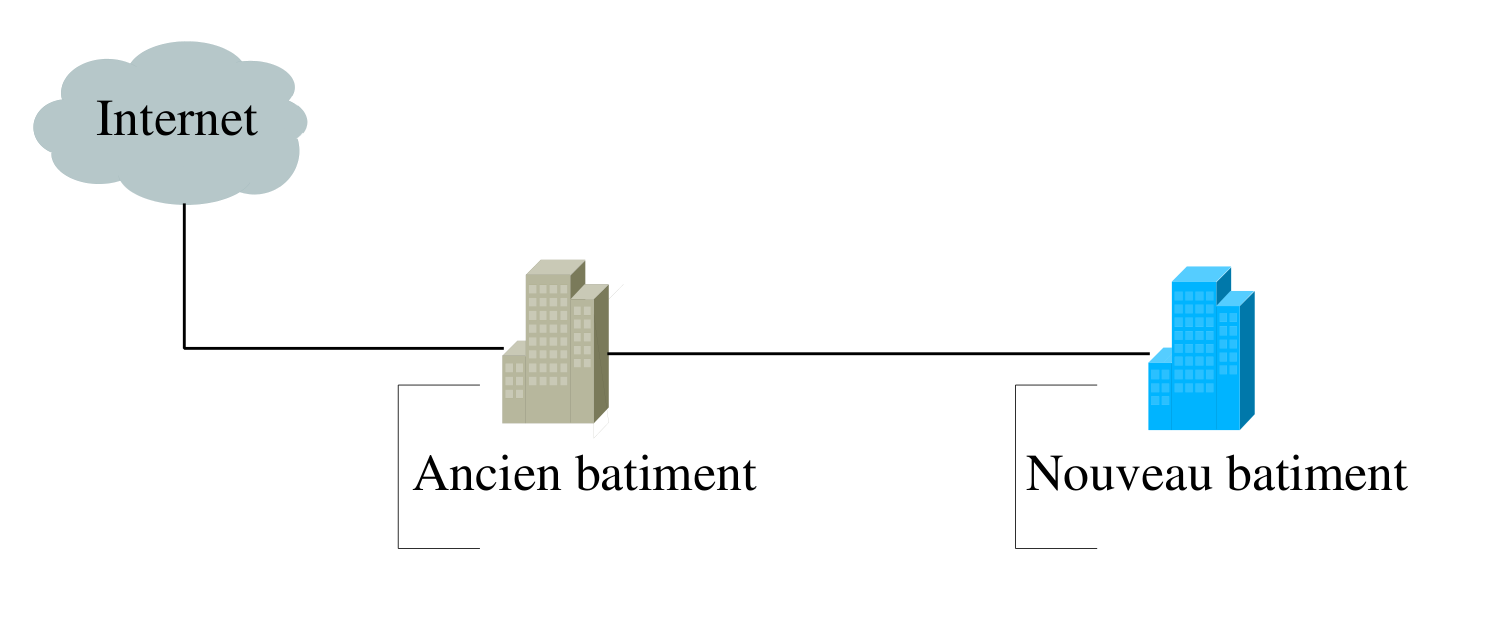
\includegraphics[width=0.8\textwidth]{./images/interco-batiment.png}
    \caption{Interconnexion du nouveau bâtiment avec l'ancien}
\end{figure}

%

L'ensemble du personnel peut communiquer via les téléphones disponible dans l'hôpital.
Dans l'enceinte du bâtiment, la connection d'équipements sans fil doit être rendu possible pour le personnel dans le cadre de leur travail.
L'accés à internet est fournit aux patients via une connection sans fil.


%
%
\subsection{Description du bâtiment}

Il est important de savoir comment le batiment est concu afin de définir les équipements et périphériques utiles au personnels et aux patients.
Ces informations seront utiles pour déterminer l'architecture du réseau.
Dans un premier temps nous allons nous intéresser aux spécificités de chaque étage et aux dimensions des locaux.

%

Le niveau -2 contient seulement un parking et les vestiaires du personnel.
Aucun accès réseau n'est nécessaire au niveau métier.
Ce niveau est aussi l'arrivée du tunnel reliant les deux bâtiments, c'est donc aussi ici que le lien d'interconnexion des deux bâtiments est installé.
Ce lien doit monter jusqu'au rez-de-chaussée afin d'atteindre une salle dédié au infrastructure du réseau.

%

Le niveau -1, qui est l'étage le plus critique car il héberge deux blocs opératoires et 4 salles d'imageries, c'est donc ici que les équipements médicaux se situent.
Ces équipements posent certaines contraintes comme par exemple des contraintes en terme de pollution électromagnétique pour les IRM.
Les ordinateurs connectés sur ces appareils sont aussi très vulnérables : ces postes tournent sous des versions obsolètes de systèmes d'exploitation.
Ils doivent donc être isolés dans le réseau et ne pas être connectés a Internet.

%

Le rez-de-chaussée, appelé par la suite niveau 0, contient une salle d'accueil, une salle d'attente, sept bureaux dédiés au personnel administratif et une salle dédiée au réseau informatique.
C'est dans cette dernière que le lien vers l'autre bâtiment sera connecté.
Cette salle contiendra donc le coeur de réseau de ce bâtiment.
Le maximum d'équipements y est aussi installer pour alléger les armoires techniques de dimensions limitées des autres étages .

%

Le premier étage (niveau 1) est composé de cinq bureaux de médecins, deux salles de réunions et deux laboratoire.
Cet étage est donc dédié uniquement au personnel de la clinique.

%

Les trois derniers étages (niveau 2 à 4) sont composés des chambres des patients.
Chaque étage comporte 15 chambres ayant chacune des dimensions avoisinant les $12 m^2$ $(4m*3m)$.

%

Enfin, à chaque étage un petit local, une armoire technique, est prévu afin de recevoir quelques équipements réseaux.


%
%
\subsection{Besoins materiels}

Il est important de connaître les technologies et périphériques nécessaires pour répondre aux besoins.
On va donc ici détailler les technologies et équipements nécessaires par étage.

%

N -2 :
Aucun accés réseau n'est nécessaire à ce niveau.
Il y a l'arrivé de la fibre reliant les deux bâtiments à ce niveau.
Cette fibre est redondée et connectée à la salle réseau (le cœur du réseau) au rez-de-chaussée.

%

N -1 :
Chaque bloc opératoires doit avoir au moins 2 prises Ethernet de type Rj45 afin d'y brancher les ordianteurs reliant les machines.
Un téléphone IP et un ordinateur sont installés dans chaque salle de préparation d'opération.
Dans les salles d’imageries un poste par salle et un téléphone IP sont nécessaires.
Les équipements médicaux sont directement reliés aux ordinateurs.

%

N 0 :
C'est à ce niveau que la salle dédiée aux infrastructures réseau est située.
On y trouve une baie, sur laquelle sont raccordés les équipements tels que les serveurs, routeurs, commutateurs et le stockage des données.
L'accueil est constitué de deux télephones IP et deux ordinateurs.
Des bornes WiFi sont présentes afin de fournir un accés réseau aux visiteurs.

%

N 1 : Les cinqs bureaux de médecin sont composés d'un télephone IP, d'un ordinateur reliés au réseau et une imprimante relié en USB directement à l'ordinateur.
Les deux salles de reunions sont composées d'un télephone IP et d'un ordinateur.
Les deux laboratoires de recherche ont un télephone IP et deux ordinateurs.
L'étage est couvert par la wifi.

%

N 2-4 : Les quinzes chambres sont équipées d'un téléphone IP fixe.
Chaque étages a deux ordinateurs et télephones Ip mis a disposition pour le personnel.
Ils sont aussi couvert par la wifi pour le personnel et pour fournir internet aux patients.

%
%




%~ On peut mettre des mots en \emph{italique},
%~ en \textsc{petites Majuscules} ou
%~ en \texttt{largeur fixe (machine à écrire)}.

%~ Voici un deuxième paragraphe avec une formule mathématique simple : $e = mc^2$.

%~ Un troisième avec des \og guillemet français \fg{}.


%~ %
%~ \subsubsection{Écrire en anglais}

%~ \foreignlanguage{english}{Do you speak French? Does anybody here speak french?}


%~ %
%~ \subsection{Listes}

%~ \begin{itemize}
%~ \item Liste classique ;
%~ \item un élément ;
%~ \item et un autre élément.
%~ \end{itemize}
%~ \vspace{\parskip} % espace entre paragraphes

%~ \begin{enumerate}
%~ \item Une liste numéroté
%~ \item deux
%~ \item trois
%~ \end{enumerate}
%~ \vspace{\parskip}

%~ \begin{description}
%~ \item[Description] C'est bien pour des définitions.
%~ \item[Deux] Ou pour faire un liste spéciale.
%~ \end{description}
%~ \vspace{\parskip}


%~ %
%~ \subsection{Références}

%~ Voici une référence à l'image de la figure \ref{latex} page \pageref{latex} et une autre vers la partie \ref{p2} page \pageref{p2}.

%~ On peut citer un livre\,\up{\cite{lpp}} et on précise les détails à la fin du rapport dans la partie références.


%~ %
%~ \subsection{Note de bas de page}

%~ Voici une note\,\footnote{Texte de bas de page} de bas de page.
%~ Une deuxième\,\footnotemark{} déclarée différemment.
%~ La même note\,\footnotemark[\value{footnote}] que précédemment.

%~ \footnotetext{Il a deux références vers cette note}


%~ %
%~ \subsection{Figure}

%~ \begin{figure}[!ht]
    %~ \center
    %~ 
\includegraphics[]{./images/LaTeX_logo.png}
    %~ \caption{latex | taille original}
    %~ \label{latex}
%~ \end{figure}

%~ \begin{figure}[!ht]
    %~ \center
    %~ 
\includegraphics[width=0.5\textwidth]{./images/LaTeX_logo.png}
    %~ \caption{latex | 50\% de la largeur de la page}
%~ \end{figure}




%~ ---------------------------------------------------------------------
%~ ---------------------------------------------------------------------
%~ ---------------------------------------------------------------------
